% Options for packages loaded elsewhere
\PassOptionsToPackage{unicode}{hyperref}
\PassOptionsToPackage{hyphens}{url}
%
\documentclass[
]{article}
\usepackage{amsmath,amssymb}
\usepackage{iftex}
\ifPDFTeX
  \usepackage[T1]{fontenc}
  \usepackage[utf8]{inputenc}
  \usepackage{textcomp} % provide euro and other symbols
\else % if luatex or xetex
  \usepackage{unicode-math} % this also loads fontspec
  \defaultfontfeatures{Scale=MatchLowercase}
  \defaultfontfeatures[\rmfamily]{Ligatures=TeX,Scale=1}
\fi
\usepackage{lmodern}
\ifPDFTeX\else
  % xetex/luatex font selection
\fi
% Use upquote if available, for straight quotes in verbatim environments
\IfFileExists{upquote.sty}{\usepackage{upquote}}{}
\IfFileExists{microtype.sty}{% use microtype if available
  \usepackage[]{microtype}
  \UseMicrotypeSet[protrusion]{basicmath} % disable protrusion for tt fonts
}{}
\makeatletter
\@ifundefined{KOMAClassName}{% if non-KOMA class
  \IfFileExists{parskip.sty}{%
    \usepackage{parskip}
  }{% else
    \setlength{\parindent}{0pt}
    \setlength{\parskip}{6pt plus 2pt minus 1pt}}
}{% if KOMA class
  \KOMAoptions{parskip=half}}
\makeatother
\usepackage{xcolor}
\usepackage[margin=1in]{geometry}
\usepackage{color}
\usepackage{fancyvrb}
\newcommand{\VerbBar}{|}
\newcommand{\VERB}{\Verb[commandchars=\\\{\}]}
\DefineVerbatimEnvironment{Highlighting}{Verbatim}{commandchars=\\\{\}}
% Add ',fontsize=\small' for more characters per line
\usepackage{framed}
\definecolor{shadecolor}{RGB}{248,248,248}
\newenvironment{Shaded}{\begin{snugshade}}{\end{snugshade}}
\newcommand{\AlertTok}[1]{\textcolor[rgb]{0.94,0.16,0.16}{#1}}
\newcommand{\AnnotationTok}[1]{\textcolor[rgb]{0.56,0.35,0.01}{\textbf{\textit{#1}}}}
\newcommand{\AttributeTok}[1]{\textcolor[rgb]{0.13,0.29,0.53}{#1}}
\newcommand{\BaseNTok}[1]{\textcolor[rgb]{0.00,0.00,0.81}{#1}}
\newcommand{\BuiltInTok}[1]{#1}
\newcommand{\CharTok}[1]{\textcolor[rgb]{0.31,0.60,0.02}{#1}}
\newcommand{\CommentTok}[1]{\textcolor[rgb]{0.56,0.35,0.01}{\textit{#1}}}
\newcommand{\CommentVarTok}[1]{\textcolor[rgb]{0.56,0.35,0.01}{\textbf{\textit{#1}}}}
\newcommand{\ConstantTok}[1]{\textcolor[rgb]{0.56,0.35,0.01}{#1}}
\newcommand{\ControlFlowTok}[1]{\textcolor[rgb]{0.13,0.29,0.53}{\textbf{#1}}}
\newcommand{\DataTypeTok}[1]{\textcolor[rgb]{0.13,0.29,0.53}{#1}}
\newcommand{\DecValTok}[1]{\textcolor[rgb]{0.00,0.00,0.81}{#1}}
\newcommand{\DocumentationTok}[1]{\textcolor[rgb]{0.56,0.35,0.01}{\textbf{\textit{#1}}}}
\newcommand{\ErrorTok}[1]{\textcolor[rgb]{0.64,0.00,0.00}{\textbf{#1}}}
\newcommand{\ExtensionTok}[1]{#1}
\newcommand{\FloatTok}[1]{\textcolor[rgb]{0.00,0.00,0.81}{#1}}
\newcommand{\FunctionTok}[1]{\textcolor[rgb]{0.13,0.29,0.53}{\textbf{#1}}}
\newcommand{\ImportTok}[1]{#1}
\newcommand{\InformationTok}[1]{\textcolor[rgb]{0.56,0.35,0.01}{\textbf{\textit{#1}}}}
\newcommand{\KeywordTok}[1]{\textcolor[rgb]{0.13,0.29,0.53}{\textbf{#1}}}
\newcommand{\NormalTok}[1]{#1}
\newcommand{\OperatorTok}[1]{\textcolor[rgb]{0.81,0.36,0.00}{\textbf{#1}}}
\newcommand{\OtherTok}[1]{\textcolor[rgb]{0.56,0.35,0.01}{#1}}
\newcommand{\PreprocessorTok}[1]{\textcolor[rgb]{0.56,0.35,0.01}{\textit{#1}}}
\newcommand{\RegionMarkerTok}[1]{#1}
\newcommand{\SpecialCharTok}[1]{\textcolor[rgb]{0.81,0.36,0.00}{\textbf{#1}}}
\newcommand{\SpecialStringTok}[1]{\textcolor[rgb]{0.31,0.60,0.02}{#1}}
\newcommand{\StringTok}[1]{\textcolor[rgb]{0.31,0.60,0.02}{#1}}
\newcommand{\VariableTok}[1]{\textcolor[rgb]{0.00,0.00,0.00}{#1}}
\newcommand{\VerbatimStringTok}[1]{\textcolor[rgb]{0.31,0.60,0.02}{#1}}
\newcommand{\WarningTok}[1]{\textcolor[rgb]{0.56,0.35,0.01}{\textbf{\textit{#1}}}}
\usepackage{graphicx}
\makeatletter
\def\maxwidth{\ifdim\Gin@nat@width>\linewidth\linewidth\else\Gin@nat@width\fi}
\def\maxheight{\ifdim\Gin@nat@height>\textheight\textheight\else\Gin@nat@height\fi}
\makeatother
% Scale images if necessary, so that they will not overflow the page
% margins by default, and it is still possible to overwrite the defaults
% using explicit options in \includegraphics[width, height, ...]{}
\setkeys{Gin}{width=\maxwidth,height=\maxheight,keepaspectratio}
% Set default figure placement to htbp
\makeatletter
\def\fps@figure{htbp}
\makeatother
\setlength{\emergencystretch}{3em} % prevent overfull lines
\providecommand{\tightlist}{%
  \setlength{\itemsep}{0pt}\setlength{\parskip}{0pt}}
\setcounter{secnumdepth}{-\maxdimen} % remove section numbering
\usepackage{fvextra}
\DefineVerbatimEnvironment{Highlighting}{Verbatim}{breaklines,commandchars=\\\{\}}
\ifLuaTeX
  \usepackage{selnolig}  % disable illegal ligatures
\fi
\usepackage{bookmark}
\IfFileExists{xurl.sty}{\usepackage{xurl}}{} % add URL line breaks if available
\urlstyle{same}
\hypersetup{
  pdftitle={COVID-19 Data Analysis},
  pdfauthor={Andrew Savala},
  hidelinks,
  pdfcreator={LaTeX via pandoc}}

\title{COVID-19 Data Analysis}
\author{Andrew Savala}
\date{2025-04-05}

\begin{document}
\maketitle

\subsection{Overview}\label{overview}

In this project I will be analyzing COVID-19 time series data from the
the Center for Systems Science and Engineering (CSSE) at Johns Hopkins
University. The data set contains daily time series summary tables,
including confirmed, deaths and recovered.

My goal is to better understand the COVID-19 pandemic and what factors
contributed to deaths in the United States.

On March 10, 2023, the Johns Hopkins Corona Virus Resource Center ceased
its collecting and reporting of global COVID-19 data.

\subsection{Import COVID-19 Data}\label{import-covid-19-data}

\begin{Shaded}
\begin{Highlighting}[]
\CommentTok{\# Read time series data from Johns Hopkins University GitHub repository}
\CommentTok{\# Raw base URL}
\NormalTok{url\_base }\OtherTok{\textless{}{-}} \StringTok{"https://raw.githubusercontent.com/CSSEGISandData/COVID{-}19/master/csse\_covid\_19\_data/csse\_covid\_19\_time\_series/"}
\NormalTok{file\_names }\OtherTok{\textless{}{-}} \FunctionTok{c}\NormalTok{(}\StringTok{"time\_series\_covid19\_confirmed\_US.csv"}\NormalTok{,}
                \StringTok{"time\_series\_covid19\_deaths\_US.csv"}\NormalTok{)}
\NormalTok{urls }\OtherTok{\textless{}{-}} \FunctionTok{str\_c}\NormalTok{(url\_base, file\_names)}

\NormalTok{us\_cases }\OtherTok{\textless{}{-}} \FunctionTok{read\_csv}\NormalTok{(urls[}\DecValTok{1}\NormalTok{], }\AttributeTok{show\_col\_types =} \ConstantTok{FALSE}\NormalTok{)}
\NormalTok{us\_deaths }\OtherTok{\textless{}{-}} \FunctionTok{read\_csv}\NormalTok{(urls[}\DecValTok{2}\NormalTok{], }\AttributeTok{show\_col\_types =} \ConstantTok{FALSE}\NormalTok{)}
\end{Highlighting}
\end{Shaded}

\subsection{Tidy and Transform Data}\label{tidy-and-transform-data}

\subsubsection{Examine Our Data}\label{examine-our-data}

Here's our raw data:

\begin{Shaded}
\begin{Highlighting}[]
\CommentTok{\# Display our raw COVID{-}19 data}
\FunctionTok{head}\NormalTok{(us\_cases)}
\end{Highlighting}
\end{Shaded}

\begin{verbatim}
## # A tibble: 6 x 1,154
##        UID iso2  iso3  code3  FIPS Admin2  Province_State Country_Region   Lat
##      <dbl> <chr> <chr> <dbl> <dbl> <chr>   <chr>          <chr>          <dbl>
## 1 84001001 US    USA     840  1001 Autauga Alabama        US              32.5
## 2 84001003 US    USA     840  1003 Baldwin Alabama        US              30.7
## 3 84001005 US    USA     840  1005 Barbour Alabama        US              31.9
## 4 84001007 US    USA     840  1007 Bibb    Alabama        US              33.0
## 5 84001009 US    USA     840  1009 Blount  Alabama        US              34.0
## 6 84001011 US    USA     840  1011 Bullock Alabama        US              32.1
## # i 1,145 more variables: Long_ <dbl>, Combined_Key <chr>, `1/22/20` <dbl>,
## #   `1/23/20` <dbl>, `1/24/20` <dbl>, `1/25/20` <dbl>, `1/26/20` <dbl>,
## #   `1/27/20` <dbl>, `1/28/20` <dbl>, `1/29/20` <dbl>, `1/30/20` <dbl>,
## #   `1/31/20` <dbl>, `2/1/20` <dbl>, `2/2/20` <dbl>, `2/3/20` <dbl>,
## #   `2/4/20` <dbl>, `2/5/20` <dbl>, `2/6/20` <dbl>, `2/7/20` <dbl>,
## #   `2/8/20` <dbl>, `2/9/20` <dbl>, `2/10/20` <dbl>, `2/11/20` <dbl>,
## #   `2/12/20` <dbl>, `2/13/20` <dbl>, `2/14/20` <dbl>, `2/15/20` <dbl>, ...
\end{verbatim}

\begin{Shaded}
\begin{Highlighting}[]
\FunctionTok{head}\NormalTok{(us\_deaths)}
\end{Highlighting}
\end{Shaded}

\begin{verbatim}
## # A tibble: 6 x 1,155
##        UID iso2  iso3  code3  FIPS Admin2  Province_State Country_Region   Lat
##      <dbl> <chr> <chr> <dbl> <dbl> <chr>   <chr>          <chr>          <dbl>
## 1 84001001 US    USA     840  1001 Autauga Alabama        US              32.5
## 2 84001003 US    USA     840  1003 Baldwin Alabama        US              30.7
## 3 84001005 US    USA     840  1005 Barbour Alabama        US              31.9
## 4 84001007 US    USA     840  1007 Bibb    Alabama        US              33.0
## 5 84001009 US    USA     840  1009 Blount  Alabama        US              34.0
## 6 84001011 US    USA     840  1011 Bullock Alabama        US              32.1
## # i 1,146 more variables: Long_ <dbl>, Combined_Key <chr>, Population <dbl>,
## #   `1/22/20` <dbl>, `1/23/20` <dbl>, `1/24/20` <dbl>, `1/25/20` <dbl>,
## #   `1/26/20` <dbl>, `1/27/20` <dbl>, `1/28/20` <dbl>, `1/29/20` <dbl>,
## #   `1/30/20` <dbl>, `1/31/20` <dbl>, `2/1/20` <dbl>, `2/2/20` <dbl>,
## #   `2/3/20` <dbl>, `2/4/20` <dbl>, `2/5/20` <dbl>, `2/6/20` <dbl>,
## #   `2/7/20` <dbl>, `2/8/20` <dbl>, `2/9/20` <dbl>, `2/10/20` <dbl>,
## #   `2/11/20` <dbl>, `2/12/20` <dbl>, `2/13/20` <dbl>, `2/14/20` <dbl>, ...
\end{verbatim}

Lets continue with looking at our US data.

\begin{Shaded}
\begin{Highlighting}[]
\CommentTok{\# Convert US cases wide to long format and drop columns we don\textquotesingle{}t care about}
\NormalTok{us\_cases\_long }\OtherTok{\textless{}{-}}\NormalTok{ us\_cases }\SpecialCharTok{\%\textgreater{}\%}
  \FunctionTok{pivot\_longer}\NormalTok{(}\AttributeTok{cols =} \SpecialCharTok{{-}}\NormalTok{(UID}\SpecialCharTok{:}\NormalTok{Combined\_Key), }
               \AttributeTok{names\_to =} \StringTok{"Date"}\NormalTok{, }\AttributeTok{values\_to =} \StringTok{"Cases"}\NormalTok{) }\SpecialCharTok{\%\textgreater{}\%}
  \FunctionTok{select}\NormalTok{(Admin2}\SpecialCharTok{:}\NormalTok{Cases) }\SpecialCharTok{\%\textgreater{}\%}
  \FunctionTok{mutate}\NormalTok{(}\AttributeTok{Date =} \FunctionTok{mdy}\NormalTok{(Date)) }\SpecialCharTok{\%\textgreater{}\%}
  \FunctionTok{select}\NormalTok{(}\SpecialCharTok{{-}}\FunctionTok{c}\NormalTok{(Lat, Long\_))}

\CommentTok{\# Do the same with the US Deaths data}
\NormalTok{us\_deaths\_long }\OtherTok{\textless{}{-}}\NormalTok{ us\_deaths }\SpecialCharTok{\%\textgreater{}\%}
  \FunctionTok{pivot\_longer}\NormalTok{(}\AttributeTok{cols =} \SpecialCharTok{{-}}\NormalTok{(UID}\SpecialCharTok{:}\NormalTok{Population),}
               \AttributeTok{names\_to =} \StringTok{"Date"}\NormalTok{, }\AttributeTok{values\_to =} \StringTok{"Deaths"}\NormalTok{) }\SpecialCharTok{\%\textgreater{}\%}
  \FunctionTok{select}\NormalTok{(Admin2}\SpecialCharTok{:}\NormalTok{Deaths) }\SpecialCharTok{\%\textgreater{}\%}
  \FunctionTok{mutate}\NormalTok{(}\AttributeTok{Date =} \FunctionTok{mdy}\NormalTok{(Date)) }\SpecialCharTok{\%\textgreater{}\%}
  \FunctionTok{select}\NormalTok{(}\SpecialCharTok{{-}}\FunctionTok{c}\NormalTok{(Lat, Long\_))}

\FunctionTok{head}\NormalTok{(us\_cases\_long)}
\end{Highlighting}
\end{Shaded}

\begin{verbatim}
## # A tibble: 6 x 6
##   Admin2  Province_State Country_Region Combined_Key         Date       Cases
##   <chr>   <chr>          <chr>          <chr>                <date>     <dbl>
## 1 Autauga Alabama        US             Autauga, Alabama, US 2020-01-22     0
## 2 Autauga Alabama        US             Autauga, Alabama, US 2020-01-23     0
## 3 Autauga Alabama        US             Autauga, Alabama, US 2020-01-24     0
## 4 Autauga Alabama        US             Autauga, Alabama, US 2020-01-25     0
## 5 Autauga Alabama        US             Autauga, Alabama, US 2020-01-26     0
## 6 Autauga Alabama        US             Autauga, Alabama, US 2020-01-27     0
\end{verbatim}

\begin{Shaded}
\begin{Highlighting}[]
\FunctionTok{head}\NormalTok{(us\_deaths\_long)}
\end{Highlighting}
\end{Shaded}

\begin{verbatim}
## # A tibble: 6 x 7
##   Admin2 Province_State Country_Region Combined_Key Population Date       Deaths
##   <chr>  <chr>          <chr>          <chr>             <dbl> <date>      <dbl>
## 1 Autau~ Alabama        US             Autauga, Al~      55869 2020-01-22      0
## 2 Autau~ Alabama        US             Autauga, Al~      55869 2020-01-23      0
## 3 Autau~ Alabama        US             Autauga, Al~      55869 2020-01-24      0
## 4 Autau~ Alabama        US             Autauga, Al~      55869 2020-01-25      0
## 5 Autau~ Alabama        US             Autauga, Al~      55869 2020-01-26      0
## 6 Autau~ Alabama        US             Autauga, Al~      55869 2020-01-27      0
\end{verbatim}

We can combine our US data.

\begin{Shaded}
\begin{Highlighting}[]
\CommentTok{\# Combine us cases and deaths data}
\NormalTok{us\_data }\OtherTok{\textless{}{-}}\NormalTok{ us\_cases\_long }\SpecialCharTok{\%\textgreater{}\%}
  \FunctionTok{full\_join}\NormalTok{(us\_deaths\_long)}
\end{Highlighting}
\end{Shaded}

\begin{verbatim}
## Joining with `by = join_by(Admin2, Province_State, Country_Region,
## Combined_Key, Date)`
\end{verbatim}

Lets filter our US data to only include states with cases greater than
0. This will help us with our analysis.

\begin{Shaded}
\begin{Highlighting}[]
\CommentTok{\# Filter US data where the cases and population are positive}
\NormalTok{us\_data }\OtherTok{\textless{}{-}}\NormalTok{ us\_data }\SpecialCharTok{\%\textgreater{}\%} \FunctionTok{filter}\NormalTok{(Cases }\SpecialCharTok{\textgreater{}} \DecValTok{0}\NormalTok{) }\SpecialCharTok{\%\textgreater{}\%} \FunctionTok{filter}\NormalTok{(Population }\SpecialCharTok{\textgreater{}} \DecValTok{0}\NormalTok{)}
\FunctionTok{summary}\NormalTok{(us\_data)}
\end{Highlighting}
\end{Shaded}

\begin{verbatim}
##     Admin2          Province_State     Country_Region     Combined_Key      
##  Length:3424407     Length:3424407     Length:3424407     Length:3424407    
##  Class :character   Class :character   Class :character   Class :character  
##  Mode  :character   Mode  :character   Mode  :character   Mode  :character  
##                                                                             
##                                                                             
##                                                                             
##       Date                Cases           Population           Deaths       
##  Min.   :2020-01-22   Min.   :      1   Min.   :      86   Min.   :    0.0  
##  1st Qu.:2020-12-27   1st Qu.:    699   1st Qu.:   11710   1st Qu.:   10.0  
##  Median :2021-09-20   Median :   2865   Median :   26830   Median :   47.0  
##  Mean   :2021-09-19   Mean   :  15559   Mean   :  106024   Mean   :  204.2  
##  3rd Qu.:2022-06-15   3rd Qu.:   9354   3rd Qu.:   69830   3rd Qu.:  138.0  
##  Max.   :2023-03-09   Max.   :3710586   Max.   :10039107   Max.   :35545.0
\end{verbatim}

\subsection{Visualizations and
Analysis}\label{visualizations-and-analysis}

Lets start with some visualizations of the US data. We will create a
plot to show the trends in cases and deaths over time in the US and then
focus in on my home state of California.

\begin{Shaded}
\begin{Highlighting}[]
\CommentTok{\# US totals by state}
\NormalTok{us\_by\_state }\OtherTok{\textless{}{-}}\NormalTok{ us\_data }\SpecialCharTok{\%\textgreater{}\%}
  \FunctionTok{group\_by}\NormalTok{(Province\_State, Country\_Region, Date) }\SpecialCharTok{\%\textgreater{}\%}
  \FunctionTok{summarise}\NormalTok{(}\AttributeTok{Cases =} \FunctionTok{sum}\NormalTok{(Cases), }\AttributeTok{Deaths =} \FunctionTok{sum}\NormalTok{(Deaths), }\AttributeTok{Population =} \FunctionTok{sum}\NormalTok{(Population)) }\SpecialCharTok{\%\textgreater{}\%}
  \FunctionTok{mutate}\NormalTok{(}\AttributeTok{Deaths\_Per\_Mil =}\NormalTok{ Deaths }\SpecialCharTok{*} \DecValTok{1000000} \SpecialCharTok{/}\NormalTok{ Population,}
         \AttributeTok{Cases\_Per\_Mil =}\NormalTok{ Cases }\SpecialCharTok{*} \DecValTok{1000000} \SpecialCharTok{/}\NormalTok{ Population) }\SpecialCharTok{\%\textgreater{}\%}
  \FunctionTok{select}\NormalTok{(Province\_State, Country\_Region, Date, Cases, Deaths, Population, Deaths\_Per\_Mil, Cases\_Per\_Mil) }\SpecialCharTok{\%\textgreater{}\%}
  \FunctionTok{ungroup}\NormalTok{()}
\end{Highlighting}
\end{Shaded}

\begin{verbatim}
## `summarise()` has grouped output by 'Province_State', 'Country_Region'. You can
## override using the `.groups` argument.
\end{verbatim}

\begin{Shaded}
\begin{Highlighting}[]
\CommentTok{\# US totals}
\NormalTok{us\_totals }\OtherTok{\textless{}{-}}\NormalTok{ us\_data }\SpecialCharTok{\%\textgreater{}\%}
  \FunctionTok{group\_by}\NormalTok{(Country\_Region, Date) }\SpecialCharTok{\%\textgreater{}\%}
  \FunctionTok{summarise}\NormalTok{(}\AttributeTok{Cases =} \FunctionTok{sum}\NormalTok{(Cases), }\AttributeTok{Deaths =} \FunctionTok{sum}\NormalTok{(Deaths), }\AttributeTok{Population =} \FunctionTok{sum}\NormalTok{(Population)) }\SpecialCharTok{\%\textgreater{}\%}
  \FunctionTok{mutate}\NormalTok{(}\AttributeTok{Deaths\_Per\_Mil =}\NormalTok{ Deaths }\SpecialCharTok{*} \DecValTok{1000000} \SpecialCharTok{/}\NormalTok{ Population,}
         \AttributeTok{Cases\_Per\_Mil =}\NormalTok{ Cases }\SpecialCharTok{*} \DecValTok{1000000} \SpecialCharTok{/}\NormalTok{ Population) }\SpecialCharTok{\%\textgreater{}\%}
  \FunctionTok{select}\NormalTok{(Country\_Region, Date, Cases, Deaths, Population, Deaths\_Per\_Mil, Cases\_Per\_Mil) }\SpecialCharTok{\%\textgreater{}\%}
  \FunctionTok{ungroup}\NormalTok{()}
\end{Highlighting}
\end{Shaded}

\begin{verbatim}
## `summarise()` has grouped output by 'Country_Region'. You can override using
## the `.groups` argument.
\end{verbatim}

\begin{Shaded}
\begin{Highlighting}[]
\CommentTok{\# Plot US totals for cases and deaths over time and filter to only show cases \textgreater{} 0.  Lets also scale Y so we can compare the trends.}
\NormalTok{us\_totals }\SpecialCharTok{\%\textgreater{}\%}
  \FunctionTok{filter}\NormalTok{(Cases }\SpecialCharTok{\textgreater{}} \DecValTok{0}\NormalTok{) }\SpecialCharTok{\%\textgreater{}\%}
  \FunctionTok{ggplot}\NormalTok{(}\FunctionTok{aes}\NormalTok{(}\AttributeTok{x =}\NormalTok{ Date, }\AttributeTok{y =}\NormalTok{ Cases)) }\SpecialCharTok{+}
  \FunctionTok{geom\_line}\NormalTok{(}\FunctionTok{aes}\NormalTok{(}\AttributeTok{y =}\NormalTok{ Cases, }\AttributeTok{color =} \StringTok{"Cases"}\NormalTok{)) }\SpecialCharTok{+}
  \FunctionTok{geom\_point}\NormalTok{(}\FunctionTok{aes}\NormalTok{(}\AttributeTok{y =}\NormalTok{ Cases, }\AttributeTok{color =} \StringTok{"Cases"}\NormalTok{)) }\SpecialCharTok{+}
  \FunctionTok{geom\_line}\NormalTok{(}\FunctionTok{aes}\NormalTok{(}\AttributeTok{y =}\NormalTok{ Deaths, }\AttributeTok{color =} \StringTok{"Deaths"}\NormalTok{)) }\SpecialCharTok{+}
  \FunctionTok{geom\_point}\NormalTok{(}\FunctionTok{aes}\NormalTok{(}\AttributeTok{y =}\NormalTok{ Deaths, }\AttributeTok{color =} \StringTok{"Deaths"}\NormalTok{)) }\SpecialCharTok{+}
  \FunctionTok{scale\_y\_log10}\NormalTok{() }\SpecialCharTok{+}
  \FunctionTok{labs}\NormalTok{(}\AttributeTok{title =} \StringTok{"US COVID{-}19 Cases and Deaths Over Time"}\NormalTok{,}
       \AttributeTok{x =} \StringTok{"Date"}\NormalTok{,}
       \AttributeTok{y =} \StringTok{"Count"}\NormalTok{) }\SpecialCharTok{+}
  \FunctionTok{scale\_color\_manual}\NormalTok{(}\AttributeTok{values =} \FunctionTok{c}\NormalTok{(}\StringTok{"Cases"} \OtherTok{=} \StringTok{"blue"}\NormalTok{, }\StringTok{"Deaths"} \OtherTok{=} \StringTok{"red"}\NormalTok{)) }\SpecialCharTok{+}
  \FunctionTok{theme\_minimal}\NormalTok{()}
\end{Highlighting}
\end{Shaded}

\begin{verbatim}
## Warning in scale_y_log10(): log-10 transformation introduced infinite values.
## log-10 transformation introduced infinite values.
\end{verbatim}

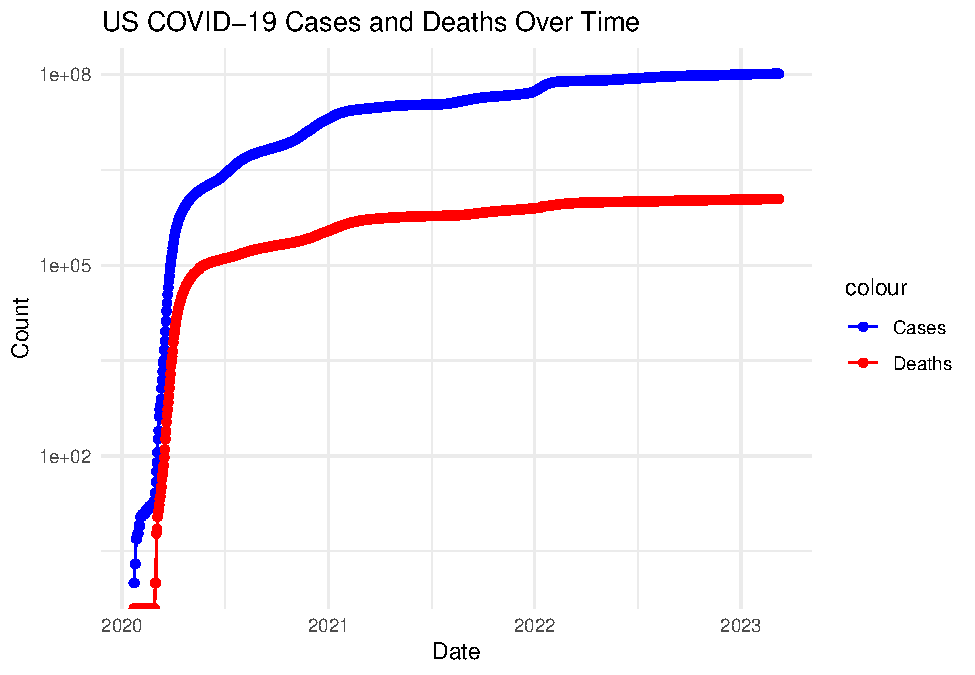
\includegraphics{covid-data-analysis_files/figure-latex/us-visualizations-1.pdf}

\begin{Shaded}
\begin{Highlighting}[]
\CommentTok{\# Now lets do the same thing, but just for the state of California}
\NormalTok{us\_by\_state }\SpecialCharTok{\%\textgreater{}\%}
  \FunctionTok{filter}\NormalTok{(Cases }\SpecialCharTok{\textgreater{}} \DecValTok{0}\NormalTok{) }\SpecialCharTok{\%\textgreater{}\%}
  \FunctionTok{filter}\NormalTok{(Province\_State }\SpecialCharTok{==} \StringTok{"California"}\NormalTok{) }\SpecialCharTok{\%\textgreater{}\%}
  \FunctionTok{ggplot}\NormalTok{(}\FunctionTok{aes}\NormalTok{(}\AttributeTok{x =}\NormalTok{ Date, }\AttributeTok{y =}\NormalTok{ Cases)) }\SpecialCharTok{+}
  \FunctionTok{geom\_line}\NormalTok{(}\FunctionTok{aes}\NormalTok{(}\AttributeTok{y =}\NormalTok{ Cases, }\AttributeTok{color =} \StringTok{"Cases"}\NormalTok{)) }\SpecialCharTok{+}
  \FunctionTok{geom\_point}\NormalTok{(}\FunctionTok{aes}\NormalTok{(}\AttributeTok{y =}\NormalTok{ Cases, }\AttributeTok{color =} \StringTok{"Cases"}\NormalTok{)) }\SpecialCharTok{+}
  \FunctionTok{geom\_line}\NormalTok{(}\FunctionTok{aes}\NormalTok{(}\AttributeTok{y =}\NormalTok{ Deaths, }\AttributeTok{color =} \StringTok{"Deaths"}\NormalTok{)) }\SpecialCharTok{+}
  \FunctionTok{geom\_point}\NormalTok{(}\FunctionTok{aes}\NormalTok{(}\AttributeTok{y =}\NormalTok{ Deaths, }\AttributeTok{color =} \StringTok{"Deaths"}\NormalTok{)) }\SpecialCharTok{+}
  \FunctionTok{scale\_y\_log10}\NormalTok{() }\SpecialCharTok{+}
  \FunctionTok{labs}\NormalTok{(}\AttributeTok{title =} \StringTok{"California COVID{-}19 Cases and Deaths Over Time"}\NormalTok{,}
       \AttributeTok{x =} \StringTok{"Date"}\NormalTok{,}
       \AttributeTok{y =} \StringTok{"Count"}\NormalTok{) }\SpecialCharTok{+}
  \FunctionTok{scale\_color\_manual}\NormalTok{(}\AttributeTok{values =} \FunctionTok{c}\NormalTok{(}\StringTok{"Cases"} \OtherTok{=} \StringTok{"blue"}\NormalTok{, }\StringTok{"Deaths"} \OtherTok{=} \StringTok{"red"}\NormalTok{)) }\SpecialCharTok{+}
  \FunctionTok{theme\_minimal}\NormalTok{()}
\end{Highlighting}
\end{Shaded}

\begin{verbatim}
## Warning in scale_y_log10(): log-10 transformation introduced infinite values.
## log-10 transformation introduced infinite values.
\end{verbatim}

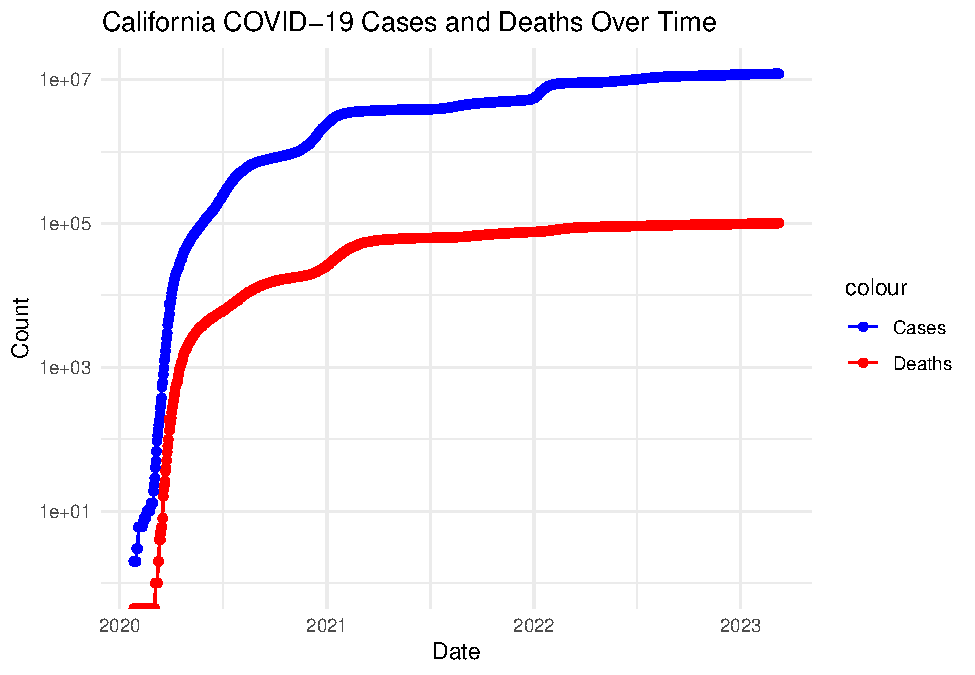
\includegraphics{covid-data-analysis_files/figure-latex/us-visualizations-2.pdf}

\subsubsection{US Analysis}\label{us-analysis}

Now lets do some analysis. We will look at the new cases and deaths over
time by week.

\begin{Shaded}
\begin{Highlighting}[]
\NormalTok{us\_totals }\OtherTok{\textless{}{-}}\NormalTok{ us\_totals }\SpecialCharTok{\%\textgreater{}\%}
  \FunctionTok{mutate}\NormalTok{(}\AttributeTok{New\_Cases =}\NormalTok{ Cases }\SpecialCharTok{{-}} \FunctionTok{lag}\NormalTok{(Cases, }\AttributeTok{default =} \DecValTok{0}\NormalTok{),}
         \AttributeTok{New\_Deaths =}\NormalTok{ Deaths }\SpecialCharTok{{-}} \FunctionTok{lag}\NormalTok{(Deaths, }\AttributeTok{default =} \DecValTok{0}\NormalTok{))}

\NormalTok{us\_totals\_weekly }\OtherTok{\textless{}{-}}\NormalTok{ us\_totals }\SpecialCharTok{\%\textgreater{}\%}
  \FunctionTok{mutate}\NormalTok{(}\AttributeTok{Week =} \FunctionTok{floor\_date}\NormalTok{(Date, }\StringTok{"week"}\NormalTok{)) }\SpecialCharTok{\%\textgreater{}\%}
  \FunctionTok{group\_by}\NormalTok{(Week) }\SpecialCharTok{\%\textgreater{}\%}
  \FunctionTok{summarise}\NormalTok{(}
    \AttributeTok{Weekly\_Cases =} \FunctionTok{sum}\NormalTok{(New\_Cases, }\AttributeTok{na.rm =} \ConstantTok{TRUE}\NormalTok{),}
    \AttributeTok{Weekly\_Deaths =} \FunctionTok{sum}\NormalTok{(New\_Deaths, }\AttributeTok{na.rm =} \ConstantTok{TRUE}\NormalTok{)}
\NormalTok{  )}

\NormalTok{us\_totals\_weekly }\SpecialCharTok{\%\textgreater{}\%}
  \FunctionTok{filter}\NormalTok{(Weekly\_Cases }\SpecialCharTok{\textgreater{}} \DecValTok{0}\NormalTok{, Weekly\_Deaths }\SpecialCharTok{\textgreater{}} \DecValTok{0}\NormalTok{) }\SpecialCharTok{\%\textgreater{}\%}
  \FunctionTok{ggplot}\NormalTok{(}\FunctionTok{aes}\NormalTok{(}\AttributeTok{x =}\NormalTok{ Week, }\AttributeTok{y =}\NormalTok{ Weekly\_Cases)) }\SpecialCharTok{+}
  \FunctionTok{geom\_line}\NormalTok{(}\FunctionTok{aes}\NormalTok{(}\AttributeTok{color =} \StringTok{"Weekly Cases"}\NormalTok{)) }\SpecialCharTok{+}
  \FunctionTok{geom\_point}\NormalTok{(}\FunctionTok{aes}\NormalTok{(}\AttributeTok{color =} \StringTok{"Weekly Cases"}\NormalTok{)) }\SpecialCharTok{+}
  \FunctionTok{geom\_line}\NormalTok{(}\FunctionTok{aes}\NormalTok{(}\AttributeTok{y =}\NormalTok{ Weekly\_Deaths, }\AttributeTok{color =} \StringTok{"Weekly Deaths"}\NormalTok{)) }\SpecialCharTok{+}
  \FunctionTok{geom\_point}\NormalTok{(}\FunctionTok{aes}\NormalTok{(}\AttributeTok{y =}\NormalTok{ Weekly\_Deaths, }\AttributeTok{color =} \StringTok{"Weekly Deaths"}\NormalTok{)) }\SpecialCharTok{+}
  \FunctionTok{scale\_y\_log10}\NormalTok{() }\SpecialCharTok{+}
  \FunctionTok{labs}\NormalTok{(}
    \AttributeTok{title =} \StringTok{"US COVID{-}19 New Cases and Deaths Over Time (Weekly Totals)"}\NormalTok{,}
    \AttributeTok{x =} \StringTok{"Week"}\NormalTok{,}
    \AttributeTok{y =} \StringTok{"Count"}
\NormalTok{  ) }\SpecialCharTok{+}
  \FunctionTok{scale\_color\_manual}\NormalTok{(}\AttributeTok{values =} \FunctionTok{c}\NormalTok{(}\StringTok{"Weekly Cases"} \OtherTok{=} \StringTok{"blue"}\NormalTok{, }\StringTok{"Weekly Deaths"} \OtherTok{=} \StringTok{"red"}\NormalTok{)) }\SpecialCharTok{+}
  \FunctionTok{theme\_minimal}\NormalTok{()}
\end{Highlighting}
\end{Shaded}

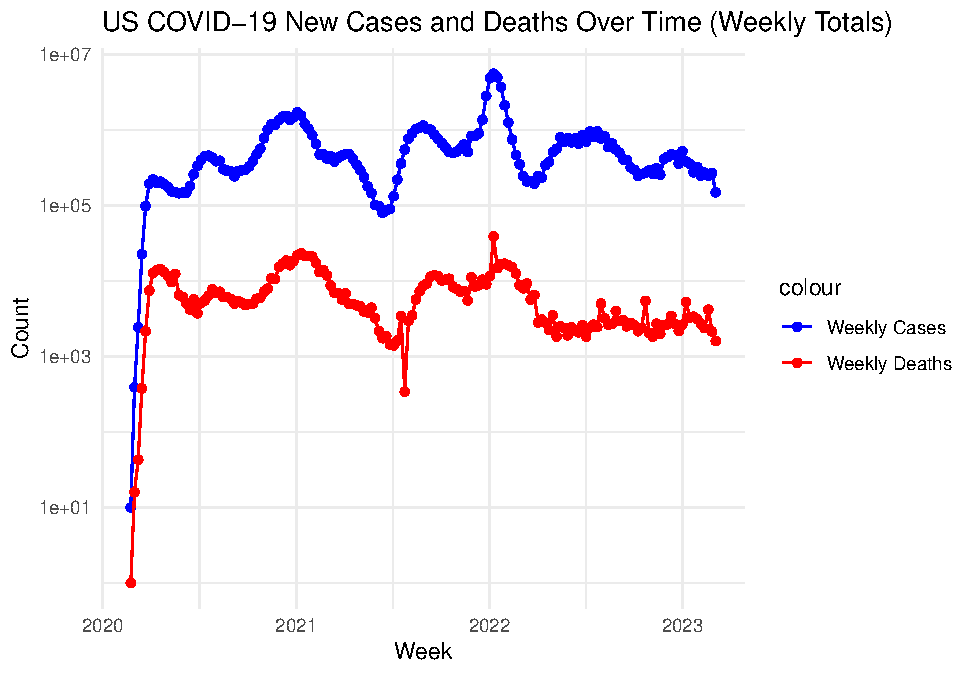
\includegraphics{covid-data-analysis_files/figure-latex/us-analysis-1.pdf}

\begin{Shaded}
\begin{Highlighting}[]
\NormalTok{us\_by\_state }\OtherTok{\textless{}{-}}\NormalTok{ us\_by\_state }\SpecialCharTok{\%\textgreater{}\%}
  \FunctionTok{mutate}\NormalTok{(}\AttributeTok{New\_Cases =}\NormalTok{ Cases }\SpecialCharTok{{-}} \FunctionTok{lag}\NormalTok{(Cases, }\AttributeTok{default =} \DecValTok{0}\NormalTok{),}
         \AttributeTok{New\_Deaths =}\NormalTok{ Deaths }\SpecialCharTok{{-}} \FunctionTok{lag}\NormalTok{(Deaths, }\AttributeTok{default =} \DecValTok{0}\NormalTok{))}

\NormalTok{ca\_totals\_weekly }\OtherTok{\textless{}{-}}\NormalTok{ us\_by\_state }\SpecialCharTok{\%\textgreater{}\%}
  \FunctionTok{filter}\NormalTok{(Province\_State }\SpecialCharTok{==} \StringTok{"California"}\NormalTok{) }\SpecialCharTok{\%\textgreater{}\%}
  \FunctionTok{mutate}\NormalTok{(}\AttributeTok{Week =} \FunctionTok{floor\_date}\NormalTok{(Date, }\StringTok{"week"}\NormalTok{)) }\SpecialCharTok{\%\textgreater{}\%}
  \FunctionTok{group\_by}\NormalTok{(Week) }\SpecialCharTok{\%\textgreater{}\%}
  \FunctionTok{summarise}\NormalTok{(}
    \AttributeTok{Weekly\_Cases =} \FunctionTok{sum}\NormalTok{(New\_Cases, }\AttributeTok{na.rm =} \ConstantTok{TRUE}\NormalTok{),}
    \AttributeTok{Weekly\_Deaths =} \FunctionTok{sum}\NormalTok{(New\_Deaths, }\AttributeTok{na.rm =} \ConstantTok{TRUE}\NormalTok{)}
\NormalTok{  )}

\NormalTok{ca\_totals\_weekly }\SpecialCharTok{\%\textgreater{}\%}
  \FunctionTok{filter}\NormalTok{(Weekly\_Cases }\SpecialCharTok{\textgreater{}} \DecValTok{0}\NormalTok{, Weekly\_Deaths }\SpecialCharTok{\textgreater{}} \DecValTok{0}\NormalTok{) }\SpecialCharTok{\%\textgreater{}\%}
  \FunctionTok{ggplot}\NormalTok{(}\FunctionTok{aes}\NormalTok{(}\AttributeTok{x =}\NormalTok{ Week, }\AttributeTok{y =}\NormalTok{ Weekly\_Cases)) }\SpecialCharTok{+}
  \FunctionTok{geom\_line}\NormalTok{(}\FunctionTok{aes}\NormalTok{(}\AttributeTok{color =} \StringTok{"Weekly Cases"}\NormalTok{)) }\SpecialCharTok{+}
  \FunctionTok{geom\_point}\NormalTok{(}\FunctionTok{aes}\NormalTok{(}\AttributeTok{color =} \StringTok{"Weekly Cases"}\NormalTok{)) }\SpecialCharTok{+}
  \FunctionTok{geom\_line}\NormalTok{(}\FunctionTok{aes}\NormalTok{(}\AttributeTok{y =}\NormalTok{ Weekly\_Deaths, }\AttributeTok{color =} \StringTok{"Weekly Deaths"}\NormalTok{)) }\SpecialCharTok{+}
  \FunctionTok{geom\_point}\NormalTok{(}\FunctionTok{aes}\NormalTok{(}\AttributeTok{y =}\NormalTok{ Weekly\_Deaths, }\AttributeTok{color =} \StringTok{"Weekly Deaths"}\NormalTok{)) }\SpecialCharTok{+}
  \FunctionTok{scale\_y\_log10}\NormalTok{() }\SpecialCharTok{+}
  \FunctionTok{labs}\NormalTok{(}
    \AttributeTok{title =} \StringTok{"California COVID{-}19 New Cases and Deaths Over Time (Weekly Totals)"}\NormalTok{,}
    \AttributeTok{x =} \StringTok{"Week"}\NormalTok{,}
    \AttributeTok{y =} \StringTok{"Count"}
\NormalTok{  ) }\SpecialCharTok{+}
  \FunctionTok{scale\_color\_manual}\NormalTok{(}\AttributeTok{values =} \FunctionTok{c}\NormalTok{(}\StringTok{"Weekly Cases"} \OtherTok{=} \StringTok{"blue"}\NormalTok{, }\StringTok{"Weekly Deaths"} \OtherTok{=} \StringTok{"red"}\NormalTok{)) }\SpecialCharTok{+}
  \FunctionTok{theme\_minimal}\NormalTok{()}
\end{Highlighting}
\end{Shaded}

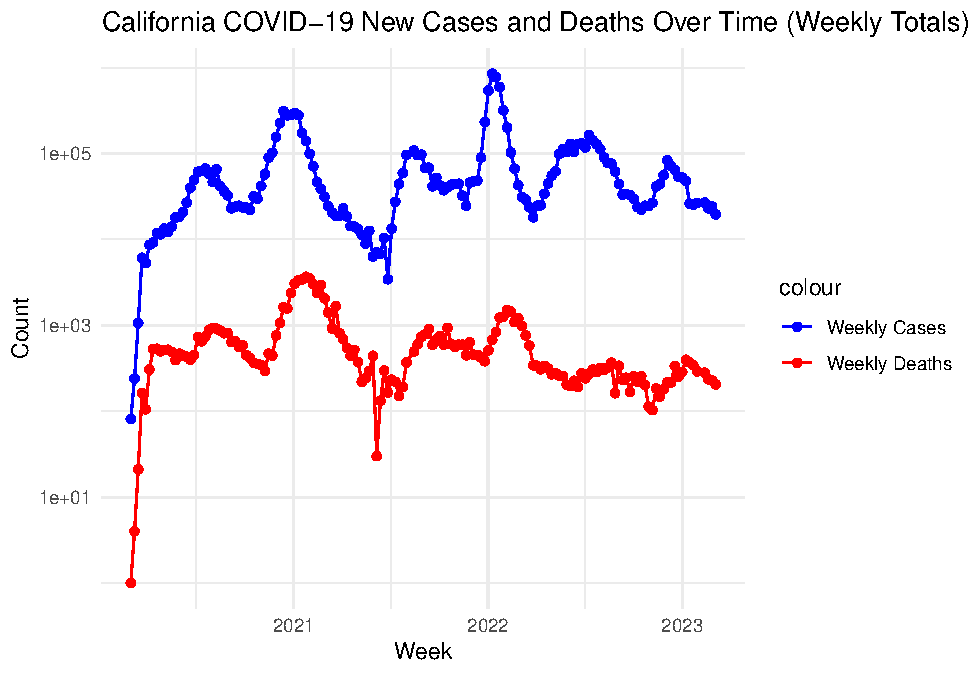
\includegraphics{covid-data-analysis_files/figure-latex/state-analysis-1.pdf}

Now lets see which states had the most deaths and cases per thousand.

\begin{Shaded}
\begin{Highlighting}[]
\CommentTok{\# Calculate cases and deaths per thousand grouped by state}
\NormalTok{us\_state\_totals }\OtherTok{\textless{}{-}}\NormalTok{ us\_by\_state }\SpecialCharTok{\%\textgreater{}\%}
  \FunctionTok{group\_by}\NormalTok{(Province\_State) }\SpecialCharTok{\%\textgreater{}\%}
  \FunctionTok{summarise}\NormalTok{(}\AttributeTok{Cases =} \FunctionTok{max}\NormalTok{(Cases), }\AttributeTok{Deaths =} \FunctionTok{max}\NormalTok{(Deaths), }
            \AttributeTok{Population =} \FunctionTok{max}\NormalTok{(Population),}
            \AttributeTok{Cases\_Per\_Thousand =} \DecValTok{1000} \SpecialCharTok{*}\NormalTok{ Cases }\SpecialCharTok{/}\NormalTok{ Population,}
            \AttributeTok{Deaths\_Per\_Thousand =} \DecValTok{1000} \SpecialCharTok{*}\NormalTok{ Deaths }\SpecialCharTok{/}\NormalTok{ Population) }\SpecialCharTok{\%\textgreater{}\%}
  \FunctionTok{filter}\NormalTok{(Cases }\SpecialCharTok{\textgreater{}} \DecValTok{0}\NormalTok{, Population }\SpecialCharTok{\textgreater{}} \DecValTok{0}\NormalTok{)}

\CommentTok{\# Find top 5 states with most Deaths\_Per\_Thousand}
\NormalTok{us\_state\_totals }\SpecialCharTok{\%\textgreater{}\%}
  \FunctionTok{arrange}\NormalTok{(}\FunctionTok{desc}\NormalTok{(Deaths\_Per\_Thousand)) }\SpecialCharTok{\%\textgreater{}\%}
  \FunctionTok{slice}\NormalTok{(}\DecValTok{1}\SpecialCharTok{:}\DecValTok{5}\NormalTok{) }\SpecialCharTok{\%\textgreater{}\%}
  \FunctionTok{ggplot}\NormalTok{(}\FunctionTok{aes}\NormalTok{(}\AttributeTok{x =} \FunctionTok{reorder}\NormalTok{(Province\_State, Deaths\_Per\_Thousand), }\AttributeTok{y =}\NormalTok{ Deaths\_Per\_Thousand)) }\SpecialCharTok{+}
  \FunctionTok{geom\_bar}\NormalTok{(}\AttributeTok{stat =} \StringTok{"identity"}\NormalTok{, }\AttributeTok{fill =} \StringTok{"red"}\NormalTok{) }\SpecialCharTok{+}
  \FunctionTok{coord\_flip}\NormalTok{() }\SpecialCharTok{+}
  \FunctionTok{labs}\NormalTok{(}\AttributeTok{title =} \StringTok{"Top 5 States with Most Deaths Per Thousand"}\NormalTok{,}
       \AttributeTok{x =} \StringTok{"State"}\NormalTok{,}
       \AttributeTok{y =} \StringTok{"Deaths Per Thousand"}\NormalTok{) }\SpecialCharTok{+}
  \FunctionTok{theme\_minimal}\NormalTok{()}
\end{Highlighting}
\end{Shaded}

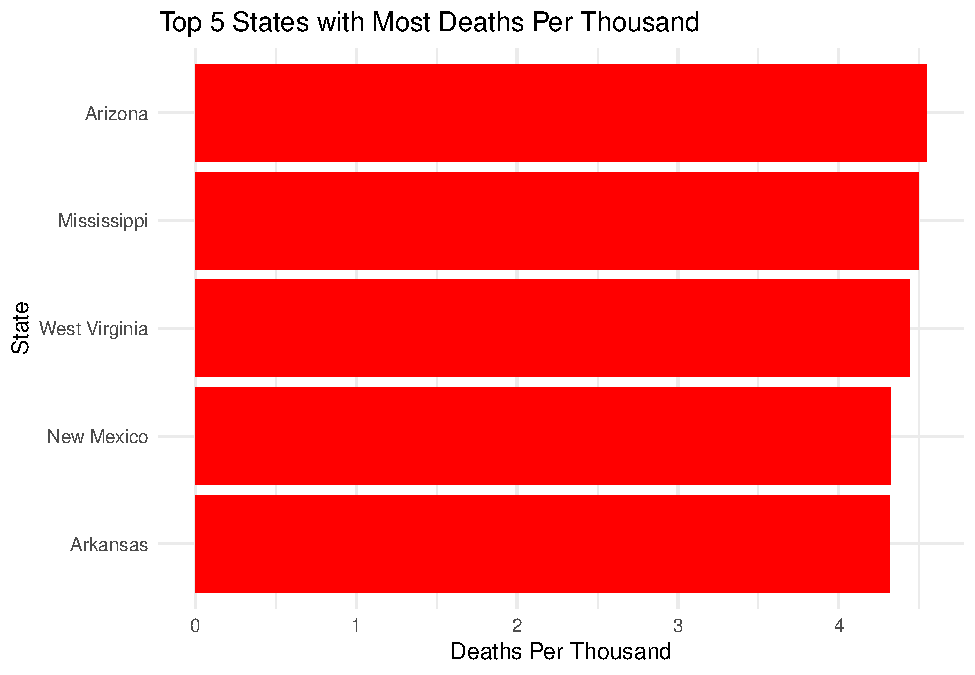
\includegraphics{covid-data-analysis_files/figure-latex/us-per-thousand-1.pdf}

\begin{Shaded}
\begin{Highlighting}[]
\CommentTok{\# Find top 5 states with most Cases\_Per\_Thousand}
\NormalTok{us\_state\_totals }\SpecialCharTok{\%\textgreater{}\%}
  \FunctionTok{arrange}\NormalTok{(}\FunctionTok{desc}\NormalTok{(Cases\_Per\_Thousand)) }\SpecialCharTok{\%\textgreater{}\%}
  \FunctionTok{slice}\NormalTok{(}\DecValTok{1}\SpecialCharTok{:}\DecValTok{5}\NormalTok{) }\SpecialCharTok{\%\textgreater{}\%}
  \FunctionTok{ggplot}\NormalTok{(}\FunctionTok{aes}\NormalTok{(}\AttributeTok{x =} \FunctionTok{reorder}\NormalTok{(Province\_State, Cases\_Per\_Thousand), }\AttributeTok{y =}\NormalTok{ Cases\_Per\_Thousand)) }\SpecialCharTok{+}
  \FunctionTok{geom\_bar}\NormalTok{(}\AttributeTok{stat =} \StringTok{"identity"}\NormalTok{, }\AttributeTok{fill =} \StringTok{"blue"}\NormalTok{) }\SpecialCharTok{+}
  \FunctionTok{coord\_flip}\NormalTok{() }\SpecialCharTok{+}
  \FunctionTok{labs}\NormalTok{(}\AttributeTok{title =} \StringTok{"Top 5 States with Most Cases Per Thousand"}\NormalTok{,}
       \AttributeTok{x =} \StringTok{"State"}\NormalTok{,}
       \AttributeTok{y =} \StringTok{"Cases Per Thousand"}\NormalTok{) }\SpecialCharTok{+}
  \FunctionTok{theme\_minimal}\NormalTok{()}
\end{Highlighting}
\end{Shaded}

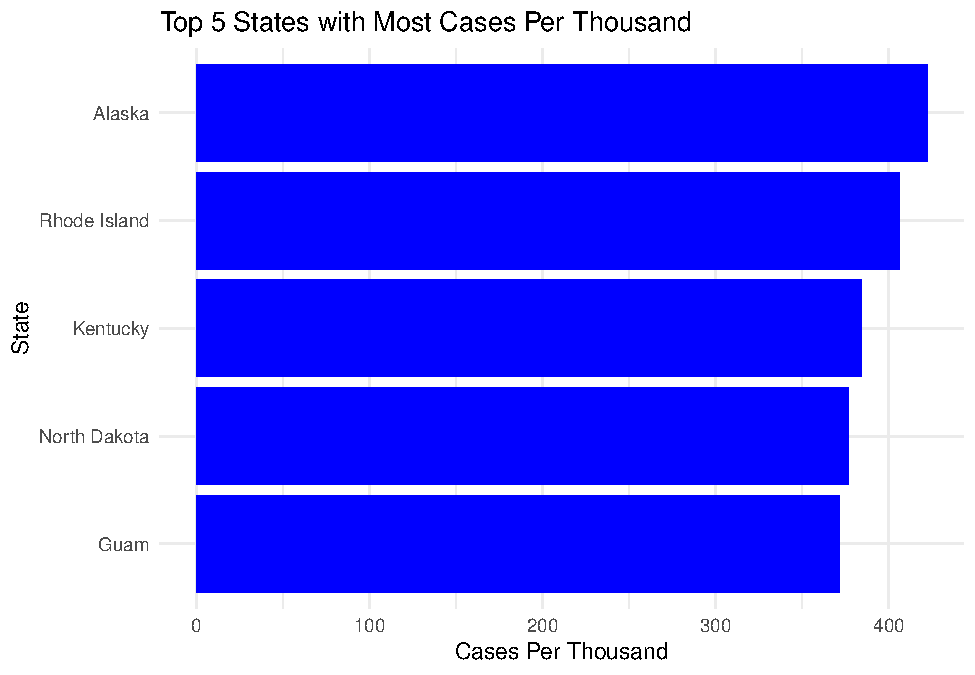
\includegraphics{covid-data-analysis_files/figure-latex/us-per-thousand-2.pdf}

\subsection{Model}\label{model}

Lets train a linear regression model to predict the number of deaths per
thousand based on the number of cases per thousand.

\subsubsection{Initial Prediction}\label{initial-prediction}

\begin{Shaded}
\begin{Highlighting}[]
\CommentTok{\# Create a linear regression model to predict deaths per thousand based on cases per thousand}
\NormalTok{model }\OtherTok{\textless{}{-}} \FunctionTok{lm}\NormalTok{(Deaths\_Per\_Thousand }\SpecialCharTok{\textasciitilde{}}\NormalTok{ Cases\_Per\_Thousand, }\AttributeTok{data =}\NormalTok{ us\_state\_totals)}
\FunctionTok{summary}\NormalTok{(model)}
\end{Highlighting}
\end{Shaded}

\begin{verbatim}
## 
## Call:
## lm(formula = Deaths_Per_Thousand ~ Cases_Per_Thousand, data = us_state_totals)
## 
## Residuals:
##     Min      1Q  Median      3Q     Max 
## -2.4231 -0.6158  0.1588  0.6722  1.2157 
## 
## Coefficients:
##                     Estimate Std. Error t value Pr(>|t|)    
## (Intercept)        -0.552774   0.762354  -0.725    0.472    
## Cases_Per_Thousand  0.011880   0.002467   4.816 1.23e-05 ***
## ---
## Signif. codes:  0 '***' 0.001 '**' 0.01 '*' 0.05 '.' 0.1 ' ' 1
## 
## Residual standard error: 0.8967 on 54 degrees of freedom
## Multiple R-squared:  0.3004, Adjusted R-squared:  0.2875 
## F-statistic: 23.19 on 1 and 54 DF,  p-value: 1.226e-05
\end{verbatim}

\begin{Shaded}
\begin{Highlighting}[]
\CommentTok{\# Lets add our predicted deaths per thousand to our data as a new column}
\NormalTok{us\_state\_totals }\OtherTok{\textless{}{-}}\NormalTok{ us\_state\_totals }\SpecialCharTok{\%\textgreater{}\%}
  \FunctionTok{mutate}\NormalTok{(}\AttributeTok{Predicted\_Deaths\_Per\_Thousand =} \FunctionTok{predict}\NormalTok{(model))}

\NormalTok{us\_state\_totals }\SpecialCharTok{\%\textgreater{}\%}
  \FunctionTok{ggplot}\NormalTok{(}\FunctionTok{aes}\NormalTok{(}\AttributeTok{x =}\NormalTok{ Cases\_Per\_Thousand, }\AttributeTok{y =}\NormalTok{ Deaths\_Per\_Thousand)) }\SpecialCharTok{+}
  \FunctionTok{geom\_point}\NormalTok{(}\FunctionTok{aes}\NormalTok{(}\AttributeTok{color =} \StringTok{"Actual Data"}\NormalTok{)) }\SpecialCharTok{+}
  \FunctionTok{geom\_line}\NormalTok{(}\FunctionTok{aes}\NormalTok{(}\AttributeTok{y =}\NormalTok{ Predicted\_Deaths\_Per\_Thousand, }\AttributeTok{color =} \StringTok{"Predicted"}\NormalTok{)) }\SpecialCharTok{+}
  \FunctionTok{labs}\NormalTok{(}\AttributeTok{title =} \StringTok{"Deaths Per Thousand vs Cases Per Thousand"}\NormalTok{,}
       \AttributeTok{x =} \StringTok{"Cases Per Thousand"}\NormalTok{,}
       \AttributeTok{y =} \StringTok{"Deaths Per Thousand"}\NormalTok{,}
       \AttributeTok{color =} \StringTok{"Legend"}\NormalTok{) }\SpecialCharTok{+}
  \FunctionTok{scale\_color\_manual}\NormalTok{(}\AttributeTok{values =} \FunctionTok{c}\NormalTok{(}\StringTok{"Actual Data"} \OtherTok{=} \StringTok{"black"}\NormalTok{, }\StringTok{"Predicted"} \OtherTok{=} \StringTok{"blue"}\NormalTok{)) }\SpecialCharTok{+}
  \FunctionTok{theme\_minimal}\NormalTok{()}
\end{Highlighting}
\end{Shaded}

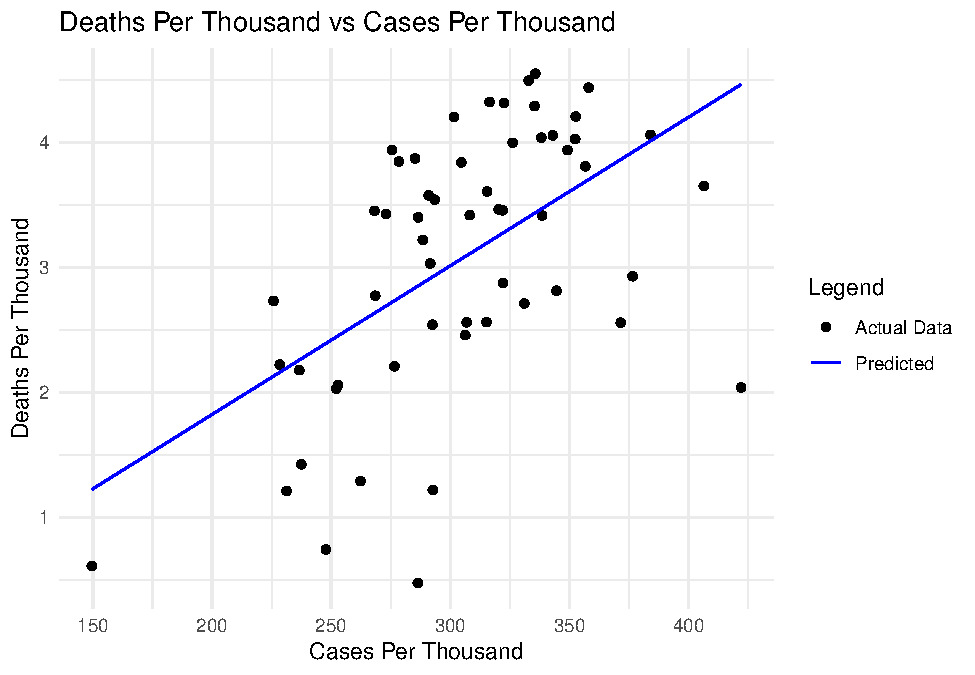
\includegraphics{covid-data-analysis_files/figure-latex/model-1.pdf}

Based on the Multiple R-squared, we can see that our model explains
about 30\% of the variation in deaths per thousand. This is not a very
good model. We can try to improve it by adding more features to our
model.

\subsubsection{Additional Features}\label{additional-features}

Lets try adding vaccination data to our model and see how that impacts
our predictions. We will use the vaccination data from GovEx GitHub
repository.

\begin{Shaded}
\begin{Highlighting}[]
\CommentTok{\# Read vaccination data from GovEx GitHub repository}
\NormalTok{vaccine\_data\_url }\OtherTok{\textless{}{-}} \StringTok{"https://raw.githubusercontent.com/govex/COVID{-}19/refs/heads/master/data\_tables/vaccine\_data/us\_data/time\_series/time\_series\_covid19\_vaccine\_us.csv"}

\CommentTok{\# Lets add the columns Doses\_admin,People\_at\_least\_one\_dose,People\_fully\_vaccinated,Total\_additional\_doses}
\NormalTok{vaccine\_data }\OtherTok{\textless{}{-}} \FunctionTok{read\_csv}\NormalTok{(vaccine\_data\_url, }\AttributeTok{show\_col\_types =} \ConstantTok{FALSE}\NormalTok{) }\SpecialCharTok{\%\textgreater{}\%}
  \FunctionTok{select}\NormalTok{(Date, Province\_State, Country\_Region, Doses\_admin, People\_at\_least\_one\_dose, People\_fully\_vaccinated, Total\_additional\_doses)}

\CommentTok{\# Find the latest vaccination totals}
\NormalTok{us\_vaccine\_totals }\OtherTok{\textless{}{-}}\NormalTok{ vaccine\_data }\SpecialCharTok{\%\textgreater{}\%}
  \FunctionTok{group\_by}\NormalTok{(Province\_State) }\SpecialCharTok{\%\textgreater{}\%}
  \FunctionTok{summarise}\NormalTok{(}
    \AttributeTok{Doses\_admin =} \FunctionTok{max}\NormalTok{(Doses\_admin, }\AttributeTok{na.rm =} \ConstantTok{TRUE}\NormalTok{),}
    \AttributeTok{People\_at\_least\_one\_dose =} \FunctionTok{max}\NormalTok{(People\_at\_least\_one\_dose, }\AttributeTok{na.rm =} \ConstantTok{TRUE}\NormalTok{),}
    \AttributeTok{People\_fully\_vaccinated =} \FunctionTok{max}\NormalTok{(People\_fully\_vaccinated, }\AttributeTok{na.rm =} \ConstantTok{TRUE}\NormalTok{),}
    \AttributeTok{Total\_additional\_doses =} \FunctionTok{max}\NormalTok{(Total\_additional\_doses, }\AttributeTok{na.rm =} \ConstantTok{TRUE}\NormalTok{)}
\NormalTok{  )}

\CommentTok{\# Join vaccine data to us state totals data}
\NormalTok{us\_state\_totals }\OtherTok{\textless{}{-}}\NormalTok{ us\_state\_totals }\SpecialCharTok{\%\textgreater{}\%}
  \FunctionTok{left\_join}\NormalTok{(us\_vaccine\_totals, }\AttributeTok{by =} \StringTok{"Province\_State"}\NormalTok{)}

\CommentTok{\# Make a per thousand column for the vaccine data}
\NormalTok{us\_state\_totals }\OtherTok{\textless{}{-}}\NormalTok{ us\_state\_totals }\SpecialCharTok{\%\textgreater{}\%}
  \FunctionTok{mutate}\NormalTok{(}
    \AttributeTok{Doses\_admin\_Per\_Thousand =} \DecValTok{1000} \SpecialCharTok{*}\NormalTok{ Doses\_admin }\SpecialCharTok{/}\NormalTok{ Population,}
    \AttributeTok{People\_at\_least\_one\_dose\_Per\_Thousand =} \DecValTok{1000} \SpecialCharTok{*}\NormalTok{ People\_at\_least\_one\_dose }\SpecialCharTok{/}\NormalTok{ Population,}
    \AttributeTok{People\_fully\_vaccinated\_Per\_Thousand =} \DecValTok{1000} \SpecialCharTok{*}\NormalTok{ People\_fully\_vaccinated }\SpecialCharTok{/}\NormalTok{ Population,}
    \AttributeTok{Total\_additional\_doses\_Per\_Thousand =} \DecValTok{1000} \SpecialCharTok{*}\NormalTok{ Total\_additional\_doses }\SpecialCharTok{/}\NormalTok{ Population}
\NormalTok{  )}
\end{Highlighting}
\end{Shaded}

Looking at our new vaccination data, we have several features to choose
from. They're likely highly correlated. Lets see how they see how they
correlate with our deaths per thousand and one another.

\begin{Shaded}
\begin{Highlighting}[]
\CommentTok{\# Correlation matrix for deaths per thousand and vaccination data}
\NormalTok{vaccine\_data }\OtherTok{\textless{}{-}}\NormalTok{ us\_state\_totals }\SpecialCharTok{\%\textgreater{}\%}
  \FunctionTok{select}\NormalTok{(Deaths\_Per\_Thousand, Cases\_Per\_Thousand, Doses\_admin\_Per\_Thousand, People\_at\_least\_one\_dose\_Per\_Thousand, People\_fully\_vaccinated\_Per\_Thousand, Total\_additional\_doses\_Per\_Thousand)}
\NormalTok{correlation\_matrix }\OtherTok{\textless{}{-}} \FunctionTok{cor}\NormalTok{(vaccine\_data, }\AttributeTok{use =} \StringTok{"pairwise.complete.obs"}\NormalTok{)}
\CommentTok{\# Plot the correlation matrix}
\CommentTok{\# corrplot(correlation\_matrix, method = "circle", type = "upper", tl.col = "black", tl.srt = 45, title = "Correlation Matrix for Deaths Per Thousand and Vaccination Data")}
\FunctionTok{corrplot}\NormalTok{(}
\NormalTok{  correlation\_matrix,}
  \AttributeTok{method =} \StringTok{"number"}\NormalTok{,        }\CommentTok{\# Show correlation coefficients}
  \AttributeTok{type =} \StringTok{"upper"}\NormalTok{,           }\CommentTok{\# Only show the upper half}
  \AttributeTok{tl.col =} \StringTok{"black"}\NormalTok{,         }\CommentTok{\# Text label color}
  \AttributeTok{tl.srt =} \DecValTok{45}\NormalTok{,              }\CommentTok{\# Rotate text labels}
  \AttributeTok{title =} \StringTok{"Correlation Matrix for Deaths Per Thousand and Vaccination Data"}\NormalTok{,}
  \AttributeTok{mar =} \FunctionTok{c}\NormalTok{(}\DecValTok{0}\NormalTok{, }\DecValTok{0}\NormalTok{, }\DecValTok{1}\NormalTok{, }\DecValTok{0}\NormalTok{),      }\CommentTok{\# Adjust margins (optional)}
  \AttributeTok{number.cex =} \FloatTok{0.8}          \CommentTok{\# Control size of the correlation coefficients}
\NormalTok{)}
\end{Highlighting}
\end{Shaded}

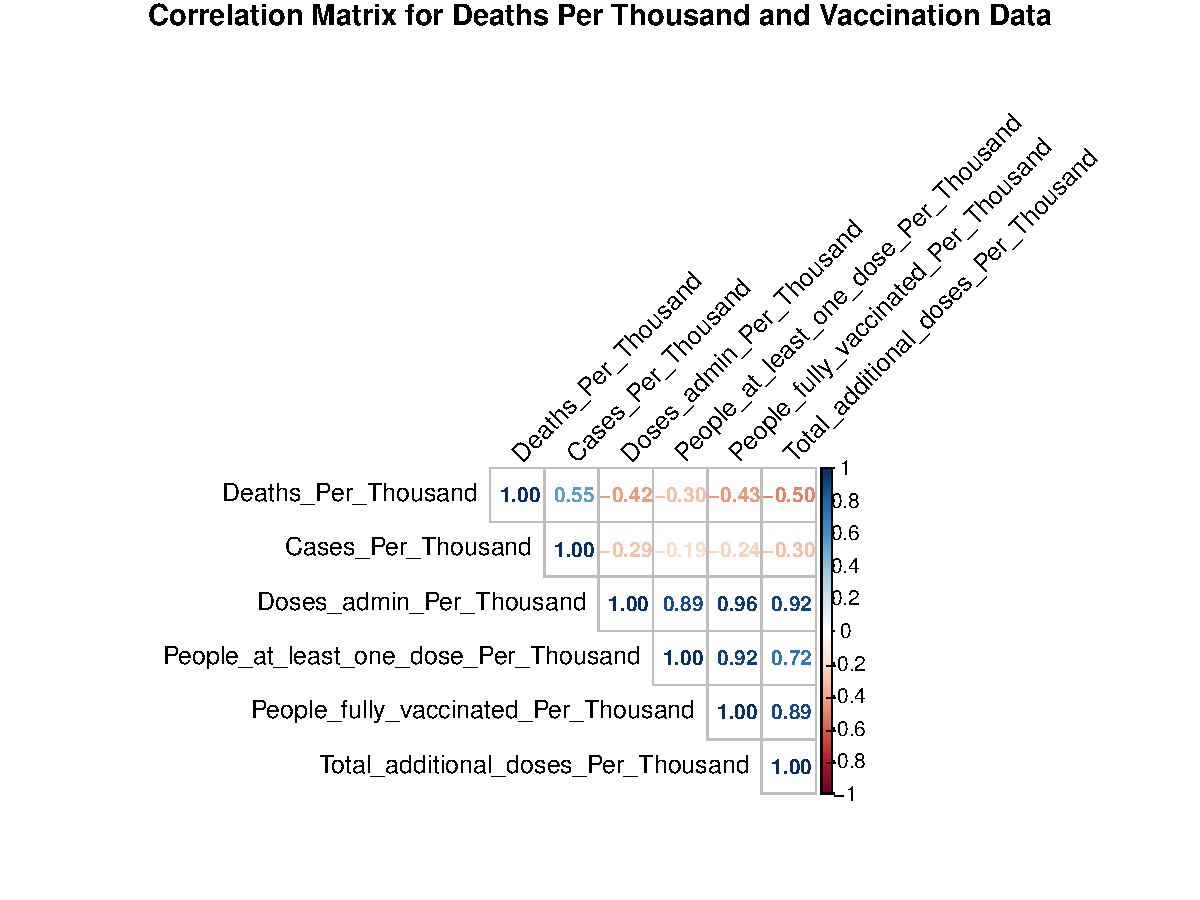
\includegraphics{covid-data-analysis_files/figure-latex/vaccine-correlation-1.pdf}
Additional doses per thousand seems to have the strongest correlation
with deaths per thousand. Lets try training a new model and add the
additional doses per thousand feature.

\begin{Shaded}
\begin{Highlighting}[]
\CommentTok{\# Create a linear regression model to predict deaths per thousand based on cases per thousand and additional doses per thousand}
\NormalTok{model\_vaccine }\OtherTok{\textless{}{-}} \FunctionTok{lm}\NormalTok{(Deaths\_Per\_Thousand }\SpecialCharTok{\textasciitilde{}}\NormalTok{ Cases\_Per\_Thousand }\SpecialCharTok{+}\NormalTok{ Total\_additional\_doses\_Per\_Thousand, }\AttributeTok{data =}\NormalTok{ us\_state\_totals)}
\FunctionTok{summary}\NormalTok{(model\_vaccine)}
\end{Highlighting}
\end{Shaded}

\begin{verbatim}
## 
## Call:
## lm(formula = Deaths_Per_Thousand ~ Cases_Per_Thousand + Total_additional_doses_Per_Thousand, 
##     data = us_state_totals)
## 
## Residuals:
##     Min      1Q  Median      3Q     Max 
## -2.2908 -0.2854  0.1337  0.5752  1.3575 
## 
## Coefficients:
##                                      Estimate Std. Error t value Pr(>|t|)    
## (Intercept)                          1.661495   0.968965   1.715 0.092241 .  
## Cases_Per_Thousand                   0.009493   0.002379   3.990 0.000204 ***
## Total_additional_doses_Per_Thousand -0.004141   0.001252  -3.308 0.001693 ** 
## ---
## Signif. codes:  0 '***' 0.001 '**' 0.01 '*' 0.05 '.' 0.1 ' ' 1
## 
## Residual standard error: 0.8241 on 53 degrees of freedom
## Multiple R-squared:  0.4202, Adjusted R-squared:  0.3983 
## F-statistic:  19.2 on 2 and 53 DF,  p-value: 5.342e-07
\end{verbatim}

\begin{Shaded}
\begin{Highlighting}[]
\CommentTok{\# Now lets compare our predicted deaths per thousand to our actual deaths per thousand}
\NormalTok{us\_state\_totals }\OtherTok{\textless{}{-}}\NormalTok{ us\_state\_totals }\SpecialCharTok{\%\textgreater{}\%}
  \FunctionTok{mutate}\NormalTok{(}\AttributeTok{Predicted\_Deaths\_Per\_Thousand\_Vaccine =} \FunctionTok{predict}\NormalTok{(model\_vaccine))}

\CommentTok{\# Now lets plot our Predicted\_Deaths\_Per\_Thousand\_Vaccine vs the actual Deaths\_Per\_Thousand}
\FunctionTok{ggplot}\NormalTok{(us\_state\_totals, }\FunctionTok{aes}\NormalTok{(}\AttributeTok{x =}\NormalTok{ Predicted\_Deaths\_Per\_Thousand\_Vaccine, }\AttributeTok{y =}\NormalTok{ Deaths\_Per\_Thousand)) }\SpecialCharTok{+}
  \FunctionTok{geom\_point}\NormalTok{(}\AttributeTok{color =} \StringTok{"blue"}\NormalTok{, }\AttributeTok{size =} \DecValTok{3}\NormalTok{) }\SpecialCharTok{+}
  \FunctionTok{geom\_abline}\NormalTok{(}\AttributeTok{intercept =} \DecValTok{0}\NormalTok{, }\AttributeTok{slope =} \DecValTok{1}\NormalTok{, }\AttributeTok{color =} \StringTok{"red"}\NormalTok{, }\AttributeTok{linetype =} \StringTok{"dashed"}\NormalTok{) }\SpecialCharTok{+}
  \FunctionTok{labs}\NormalTok{(}\AttributeTok{x =} \StringTok{"Predicted Deaths Per Thousand (Vaccine)"}\NormalTok{,}
       \AttributeTok{y =} \StringTok{"Actual Deaths Per Thousand"}\NormalTok{,}
       \AttributeTok{title =} \StringTok{"Predicted vs Actual Deaths Per Thousand"}\NormalTok{) }\SpecialCharTok{+}
  \FunctionTok{theme\_minimal}\NormalTok{()}
\end{Highlighting}
\end{Shaded}

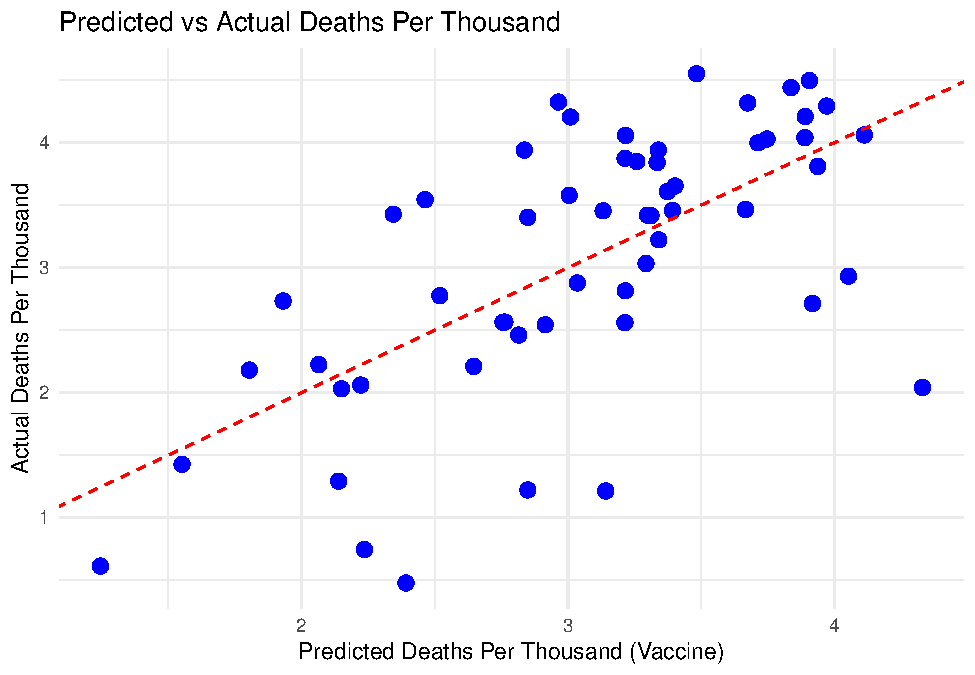
\includegraphics{covid-data-analysis_files/figure-latex/model-with-vaccine-1.pdf}

We're going in the right direction because Multiple R-squared indicates
our model explains about 42\% of the variation in deaths per thousand.
This is a significant improvement over our previous model.

\subsection{Bias Identification and
Conclusion}\label{bias-identification-and-conclusion}

Regarding bias, it's important to recognize that different states may
have different criteria for attributing deaths to COVID-19. Some may
report more conservatively, while others more liberally. This could lead
to bias in our model and our predictions. Additionally, the data is not
perfect and there may be missing or inaccurate data points. This could
also lead to bias in our model and our predictions.

In conclusion, we were able to train a model which was able to explain
roughly 42\% of the variation in deaths per thousand. We were able to do
this by adding additional features to our model, specifically
vaccination data. This is a significant improvement over our previous
model which only explained about 30\% of the variation in deaths per
thousand.

We can see that the model is not perfect, but it does provide some
insight into the relationship between cases per thousand and deaths per
thousand.

\subsection{Session Info}\label{session-info}

Record our session info for reproducibility.

\begin{Shaded}
\begin{Highlighting}[]
\FunctionTok{sessionInfo}\NormalTok{()}
\end{Highlighting}
\end{Shaded}

\begin{verbatim}
## R version 4.4.3 (2025-02-28 ucrt)
## Platform: x86_64-w64-mingw32/x64
## Running under: Windows 11 x64 (build 26100)
## 
## Matrix products: default
## 
## 
## locale:
## [1] LC_COLLATE=English_United States.utf8 
## [2] LC_CTYPE=English_United States.utf8   
## [3] LC_MONETARY=English_United States.utf8
## [4] LC_NUMERIC=C                          
## [5] LC_TIME=English_United States.utf8    
## 
## time zone: America/Los_Angeles
## tzcode source: internal
## 
## attached base packages:
## [1] stats     graphics  grDevices utils     datasets  methods   base     
## 
## other attached packages:
##  [1] forcats_1.0.0   stringr_1.5.1   dplyr_1.1.4     purrr_1.0.4    
##  [5] readr_2.1.5     tidyr_1.3.1     tibble_3.2.1    ggplot2_3.5.1  
##  [9] tidyverse_2.0.0 corrplot_0.95   lubridate_1.9.4
## 
## loaded via a namespace (and not attached):
##  [1] bit_4.6.0         gtable_0.3.6      crayon_1.5.3      compiler_4.4.3   
##  [5] tidyselect_1.2.1  parallel_4.4.3    scales_1.3.0      yaml_2.3.10      
##  [9] fastmap_1.2.0     R6_2.6.1          labeling_0.4.3    generics_0.1.3   
## [13] curl_6.2.1        knitr_1.49        munsell_0.5.1     pillar_1.10.1    
## [17] tzdb_0.4.0        rlang_1.1.5       utf8_1.2.4        stringi_1.8.4    
## [21] xfun_0.51         bit64_4.6.0-1     timechange_0.3.0  cli_3.6.4        
## [25] withr_3.0.2       magrittr_2.0.3    digest_0.6.37     grid_4.4.3       
## [29] vroom_1.6.5       rstudioapi_0.17.1 hms_1.1.3         lifecycle_1.0.4  
## [33] vctrs_0.6.5       evaluate_1.0.3    glue_1.8.0        farver_2.1.2     
## [37] colorspace_2.1-1  rmarkdown_2.29    tools_4.4.3       pkgconfig_2.0.3  
## [41] htmltools_0.5.8.1
\end{verbatim}

\end{document}
